\section{Methods}
\label{sec:design}

\begin{figure}[t]
\centering
\includegraphics[page=2,trim=0 631 18 0,clip,width=\textwidth]{figures/humanscore_figures.pdf}
\caption{Method and main result. (A) A model RDM (hidden states of all layers, z-scored and concatenated; or surprisal) and a human RDM (here, whole-brain responses per word) are computed over the same words. The score is the held-out log-likelihood gained by adding the model RDM to a regression of the human RDM on word-length and frequency RDMs. (B) Brain similarity against behavioral similarity for 118 models: median over the eight neural datasets and over the 16 reading measures of the score divided by each dataset's split-half reference. Colors: model groups; marker size: parameter count; black line: Pareto front.}
\label{fig:method}
\end{figure}

\subsection{Models}
\label{sec:design-models}

We evaluate 118 frozen, publicly released models in a $2\times2$ design that crosses a memory factor $M$ (an architecture that limits access to the preceding context) with a data factor $D$ (training on 10--100M words instead of web-scale text; Table~\ref{tab:models}, Appendix~\ref{app:models}). \textbf{Standard LLMs} ($M{=}D{=}0$; 59 models, 14M--66B parameters) are off-the-shelf web-scale models: GPT-2, GPT-Neo, OPT, Pythia, OLMo-2, Qwen3, Llama-3, Ministral, the state-space and recurrent models Mamba, Mamba-2 and RWKV-4, and the full-attention baselines of the Forgetting Transformer. \textbf{Memory-Constrained} models ($M{=}1,D{=}0$; 24 models, 15M--7.1B) use ALiBi distance penalties, forget gates, stick-breaking attention, hard 2-, 3- or 5-token windows, or a bounded recurrent state (CBR-RNN), and include web-scale models built on these mechanisms (BLOOM, Forgetting Transformer, MoLM). \textbf{BabyLM} models ($M{=}0,D{=}1$; 11 models, 33M--140M) are standard architectures from the BabyLM Challenge. \textbf{Constrained-BabyLM} models ($M{=}D{=}1$; 24 models, 15M--48M) are the small memory-constrained architectures trained on the BabyLM corpora. The groups differ by orders of magnitude in size and perplexity, which the regression below adjusts for.

\subsection{Human data}
\label{sec:design-data}

We use 15 public datasets, split into 24 dataset units (Table~\ref{tab:datasets}, Appendix~\ref{app:datasets}). \textbf{Behavior} (16 units): self-paced reading in Natural Stories \citep{futrell2021natural} and UCL Reading \citep{frank2013reading}, and eye-tracking in GECO \citep{cop2017geco}, Provo \citep{luke2018provo}, MECO \citep{siegelman2022meco}, OneStop \citep{berzak2025onestop} and ZuCo \citep{hollenstein2018zuco}, where first-pass, go-past and total reading times and the three ZuCo tasks are separate units. \textbf{Brain} (8 units): fMRI responses to sentences \citep{pereira2018toward,tuckute2024driving}, EEG during audiobook listening \citep{broderick2018electrophysiological}, N400 amplitudes in three cloze-manipulation studies \citep{nieuwland2018largescale,federmeier2007multiple,szewczyk2022context}, MEG during story listening \citep{gwilliams2022neural}, and ECoG during a podcast \citep{zada2025podcast}.

\subsection{Representational similarity score}
\label{sec:design-rdms}

\paragraph{Dissimilarity matrices.} For the multichannel recordings (Podcast, MEG-MASC, Broderick, Pereira), the response to a word (Pereira: a sentence) concatenates all participants' channels and, for time-resolved data, all samples from 0 to 600\,ms after onset; Podcast and Pereira are restricted to the language network (158 electrodes in language regions; the language-atlas voxels). Each feature is z-scored and dissimilarity is one minus the Pearson correlation. For single-response datasets (the language-network regions of Tuckute, N400 amplitudes) and for reading times, averaged over participants, the dissimilarity of two items is the absolute difference of their means; Tuckute and the N400 datasets are scored per region or electrode group and summarized by the median over units. The model RDM for brain similarity uses the hidden states of all layers except the input embedding, each feature z-scored \citep{timkey2021allbark} and concatenated, which applies one rule to models of 1 to 65 layers without layer selection. For behavioral similarity it is the absolute difference in surprisal, the model quantity that indexes processing difficulty \citep{hale2001probabilistic,levy2008expectation}. Appendix~\ref{app:same-predictor} uses one quantity on both axes.

\paragraph{RDM regression.} Let $y$ be the human dissimilarities over word pairs, $m$ the model dissimilarities and $c_1,c_2$ the absolute differences in word length and Zipf frequency. We compare
\begin{equation}
\text{base: } y_{ij} = b_0 + b_1 c_{1,ij} + b_2 c_{2,ij} + \varepsilon_{ij}, \qquad \text{full: } y_{ij} = b_0 + b_1 c_{1,ij} + b_2 c_{2,ij} + b_3 m_{ij} + \varepsilon_{ij},
\label{eq:rdmreg}
\end{equation}
and score a model by the held-out log-likelihood gain per pair, $\Delta\ell=(\ell^{\mathrm{test}}_{\mathrm{full}}-\ell^{\mathrm{test}}_{\mathrm{base}})/n_{\mathrm{test}}$. Stimuli, not pairs, are split into five folds, so test pairs never share a word with training pairs \citep{schutt2023statistical}; scores are averaged over 10 partitions, identical for all models. A model adding nothing beyond length and frequency scores 0, and since the model enters through one weight, the score does not grow with model width.

\paragraph{Normalization.} Each score is divided by a split-half reference computed with the same pairs, folds and confounds, in which the RDM of a random half of the participants replaces the model RDM to predict the other half \citep{timkey2026dissociation}. \emph{Behavioral similarity} is the median of a model's normalized scores over the 16 reading measures and \emph{brain similarity} over the eight neural datasets. A model is on the Pareto front if no other model is at least as similar on both axes and strictly more on one.

\subsection{Matched-scale regression}
\label{sec:design-stats}

For each domain we regress the normalized score $Y_{ij}$ of model $i$ on dataset unit $j$ on the constraints, size and perplexity:
\begin{equation}
Y_{ij}=\beta_0+\beta_M M_i+\beta_D D_i+\beta_{MD}M_iD_i+\beta_S\log_{10}P_i+\beta_P\log_{10}\mathrm{PPL}_{ij}+u_j+v_{\ell(i)}+\epsilon_{ij},
\label{eq:group}
\end{equation}
where $P_i$ is the parameter count, $\mathrm{PPL}_{ij}$ the perplexity of model $i$ on the text of unit $j$ (the exponential of its mean word surprisal over the unit's words, from the same pass that gives the surprisal RDMs; on Tuckute and the N400 datasets, over their sentences), and $u_j$ and $v_{\ell(i)}$ random intercepts for the dataset unit and for the model's lineage (its family, e.g.\ all Pythia sizes; each BabyLM submission is its own lineage; 26 lineages). Standard LLMs are the reference, so $\beta_M$ and $\beta_D$ compare Memory-Constrained and BabyLM models with Standard LLMs of the same size and perplexity, and $\beta_M+\beta_D+\beta_{MD}$ does so for Constrained-BabyLM models. With the lineage intercept, the constraint effects are tested against the variation between model families rather than between sizes of one family. The 26 lineages comprise 12 with Standard LLMs, 10 with Memory-Constrained, 5 with BabyLM and 6 with Constrained-BabyLM models; six memory-constrained architectures are trained on both web-scale and BabyLM data. Fits use REML (\texttt{lme4}) with Satterthwaite $t$-tests (1,870 behavioral and 934 neural rows); no fit is singular (variance components in Appendix~\ref{app:implementation}). The groups differ in other respects too, so the coefficients are adjusted associations, not causal effects.

Constrained models reach perplexities that few Standard LLMs have. To check that the adjustment does not rest on extrapolation, we add the intermediate checkpoints of the ten Pythia models (steps 128 to 128{,}000) and of the BabyLM GPT-2 baseline (1M to 1B words), 119 checkpoints in total, with an additional random intercept for the training run (Appendix~\ref{app:checkpoints}).

\subsection{Where could an advantage come from?}
\label{sec:design-dlt}

\paragraph{Word-pair bins.} The held-out $\Delta\ell$ is a sum over test pairs, so it can be split into bins of word pairs without refitting; the human references are split the same way. We use two word classes. \emph{Syntactic memory load}: Dependency Locality Theory (DLT) integration cost \citep{gibson2000dlt}, computed from a dependency parse; a word is \emph{easy} with cost 0 and \emph{hard} with cost $\geq2$, i.e.\ when it closes a dependency across at least one intervening discourse referent. We compare easy--easy pairs with pairs containing at least one hard word (\emph{any-hard}) on Natural Stories and Podcast, the two datasets in which hard words elicit a larger human response beyond length and frequency (Appendix~\ref{app:wordclass-dlt}). \emph{Word frequency}: a word is \emph{frequent} with Zipf frequency $\geq4$ and \emph{rare} with Zipf $\leq3$ \citep{vanheuven2014subtlex}; we compare frequent--frequent with \emph{any-rare} pairs on the datasets with at least 100 rare words, the 9 reading measures of GECO, OneStop, Natural Stories and ZuCo and Podcast. In both analyses, both bins are divided by the all-pairs reference of the unit, so that bins share one denominator and a bin's score is its share of the unit's reliable signal. Equation~\ref{eq:group} is fitted with every fixed effect interacted with the bin, so the interaction tests whether an association differs between bins; the random intercepts are those of the main fit, for lineage, lineage by bin and (for the 9 reading measures) measure by bin.

\paragraph{Multiple-demand network.} We rescore the three neural datasets in which the MD network can be delineated, keeping everything else fixed: the MD atlas voxels of Pereira \citep{pereira2018toward}, the MD functional regions of Tuckute (bilateral network mean; language: left-hemisphere network mean), and the word-responsive Podcast electrodes outside the language regions that lie within 10\,mm of a voxel with MD probability $\geq.1$ in a probabilistic MD map built from localizer data of 691 participants \citep{lipkin2022probabilistic}. The MD split-half references are 3--15 times smaller than the language ones and too noisy to divide by, so the outcome is each model's percentile rank among the 118 models within a dataset and network. Equation~\ref{eq:group} with dataset fixed effects and the lineage random intercept is fitted per network and pooled with all fixed effects interacted with the network.

\paragraph{Robustness.} The all-datasets fits are repeated with the per-unit robust $z$ score of the raw $\Delta\ell$ as outcome, which involves no reference (Table~\ref{tab:summary-z}); the two-dataset analysis of Natural Stories and Podcast alone is in Appendix~\ref{app:two-datasets}.
